% Options for packages loaded elsewhere
\PassOptionsToPackage{unicode}{hyperref}
\PassOptionsToPackage{hyphens}{url}
\PassOptionsToPackage{dvipsnames,svgnames,x11names}{xcolor}
%
\documentclass[
  letterpaper,
  DIV=11,
  numbers=noendperiod]{scrartcl}

\usepackage{amsmath,amssymb}
\usepackage{iftex}
\ifPDFTeX
  \usepackage[T1]{fontenc}
  \usepackage[utf8]{inputenc}
  \usepackage{textcomp} % provide euro and other symbols
\else % if luatex or xetex
  \usepackage{unicode-math}
  \defaultfontfeatures{Scale=MatchLowercase}
  \defaultfontfeatures[\rmfamily]{Ligatures=TeX,Scale=1}
\fi
\usepackage{lmodern}
\ifPDFTeX\else  
    % xetex/luatex font selection
\fi
% Use upquote if available, for straight quotes in verbatim environments
\IfFileExists{upquote.sty}{\usepackage{upquote}}{}
\IfFileExists{microtype.sty}{% use microtype if available
  \usepackage[]{microtype}
  \UseMicrotypeSet[protrusion]{basicmath} % disable protrusion for tt fonts
}{}
\makeatletter
\@ifundefined{KOMAClassName}{% if non-KOMA class
  \IfFileExists{parskip.sty}{%
    \usepackage{parskip}
  }{% else
    \setlength{\parindent}{0pt}
    \setlength{\parskip}{6pt plus 2pt minus 1pt}}
}{% if KOMA class
  \KOMAoptions{parskip=half}}
\makeatother
\usepackage{xcolor}
\setlength{\emergencystretch}{3em} % prevent overfull lines
\setcounter{secnumdepth}{-\maxdimen} % remove section numbering
% Make \paragraph and \subparagraph free-standing
\ifx\paragraph\undefined\else
  \let\oldparagraph\paragraph
  \renewcommand{\paragraph}[1]{\oldparagraph{#1}\mbox{}}
\fi
\ifx\subparagraph\undefined\else
  \let\oldsubparagraph\subparagraph
  \renewcommand{\subparagraph}[1]{\oldsubparagraph{#1}\mbox{}}
\fi


\providecommand{\tightlist}{%
  \setlength{\itemsep}{0pt}\setlength{\parskip}{0pt}}\usepackage{longtable,booktabs,array}
\usepackage{calc} % for calculating minipage widths
% Correct order of tables after \paragraph or \subparagraph
\usepackage{etoolbox}
\makeatletter
\patchcmd\longtable{\par}{\if@noskipsec\mbox{}\fi\par}{}{}
\makeatother
% Allow footnotes in longtable head/foot
\IfFileExists{footnotehyper.sty}{\usepackage{footnotehyper}}{\usepackage{footnote}}
\makesavenoteenv{longtable}
\usepackage{graphicx}
\makeatletter
\def\maxwidth{\ifdim\Gin@nat@width>\linewidth\linewidth\else\Gin@nat@width\fi}
\def\maxheight{\ifdim\Gin@nat@height>\textheight\textheight\else\Gin@nat@height\fi}
\makeatother
% Scale images if necessary, so that they will not overflow the page
% margins by default, and it is still possible to overwrite the defaults
% using explicit options in \includegraphics[width, height, ...]{}
\setkeys{Gin}{width=\maxwidth,height=\maxheight,keepaspectratio}
% Set default figure placement to htbp
\makeatletter
\def\fps@figure{htbp}
\makeatother

\KOMAoption{captions}{tableheading,figureheading}
\makeatletter
\makeatother
\makeatletter
\makeatother
\makeatletter
\@ifpackageloaded{caption}{}{\usepackage{caption}}
\AtBeginDocument{%
\ifdefined\contentsname
  \renewcommand*\contentsname{Tabla de contenidos}
\else
  \newcommand\contentsname{Tabla de contenidos}
\fi
\ifdefined\listfigurename
  \renewcommand*\listfigurename{Listado de Figuras}
\else
  \newcommand\listfigurename{Listado de Figuras}
\fi
\ifdefined\listtablename
  \renewcommand*\listtablename{Listado de Tablas}
\else
  \newcommand\listtablename{Listado de Tablas}
\fi
\ifdefined\figurename
  \renewcommand*\figurename{Figura}
\else
  \newcommand\figurename{Figura}
\fi
\ifdefined\tablename
  \renewcommand*\tablename{Tabla}
\else
  \newcommand\tablename{Tabla}
\fi
}
\@ifpackageloaded{float}{}{\usepackage{float}}
\floatstyle{ruled}
\@ifundefined{c@chapter}{\newfloat{codelisting}{h}{lop}}{\newfloat{codelisting}{h}{lop}[chapter]}
\floatname{codelisting}{Listado}
\newcommand*\listoflistings{\listof{codelisting}{Listado de Listados}}
\makeatother
\makeatletter
\@ifpackageloaded{caption}{}{\usepackage{caption}}
\@ifpackageloaded{subcaption}{}{\usepackage{subcaption}}
\makeatother
\makeatletter
\@ifpackageloaded{tcolorbox}{}{\usepackage[skins,breakable]{tcolorbox}}
\makeatother
\makeatletter
\@ifundefined{shadecolor}{\definecolor{shadecolor}{rgb}{.97, .97, .97}}
\makeatother
\makeatletter
\makeatother
\makeatletter
\makeatother
\ifLuaTeX
\usepackage[bidi=basic]{babel}
\else
\usepackage[bidi=default]{babel}
\fi
\babelprovide[main,import]{spanish}
% get rid of language-specific shorthands (see #6817):
\let\LanguageShortHands\languageshorthands
\def\languageshorthands#1{}
\ifLuaTeX
  \usepackage{selnolig}  % disable illegal ligatures
\fi
\usepackage[]{biblatex}
\addbibresource{../../../../references.bib}
\IfFileExists{bookmark.sty}{\usepackage{bookmark}}{\usepackage{hyperref}}
\IfFileExists{xurl.sty}{\usepackage{xurl}}{} % add URL line breaks if available
\urlstyle{same} % disable monospaced font for URLs
\hypersetup{
  pdftitle={El Mercado Relevante Industrial de Bienes y el Mercado Geográfico},
  pdfauthor={Edison Achalma Mendoza},
  pdflang={es},
  colorlinks=true,
  linkcolor={blue},
  filecolor={Maroon},
  citecolor={Blue},
  urlcolor={Blue},
  pdfcreator={LaTeX via pandoc}}

\title{El Mercado Relevante Industrial de Bienes y el Mercado
Geográfico}
\usepackage{etoolbox}
\makeatletter
\providecommand{\subtitle}[1]{% add subtitle to \maketitle
  \apptocmd{\@title}{\par {\large #1 \par}}{}{}
}
\makeatother
\subtitle{Explorando las Implicaciones Teóricas y Prácticas del Mercado
Relevante en la Industria de Bienes. Perspectivas y Desafíos}
\author{Edison Achalma Mendoza}
\date{2023-06-15}

\begin{document}
\maketitle
\ifdefined\Shaded\renewenvironment{Shaded}{\begin{tcolorbox}[frame hidden, boxrule=0pt, interior hidden, borderline west={3pt}{0pt}{shadecolor}, breakable, enhanced, sharp corners]}{\end{tcolorbox}}\fi

\hypertarget{sistema-econuxf3mio-y-mercado}{%
\section{Sistema económio y
mercado}\label{sistema-econuxf3mio-y-mercado}}

\hypertarget{sistema-econuxf3mico}{%
\subsection{Sistema económico}\label{sistema-econuxf3mico}}

El sistema económico se refiere a la forma en que se organiza y dirige
la actividad económica de un país, abarcando aspectos sociales,
políticos, económicos y jurídicos. Define cómo se producirán y
distribuirán los bienes y servicios, así como la asignación de los
recursos escasos para su producción. Además, incluye la organización
política, la regulación e intervención del estado, y el marco jurídico
que rige las transacciones económicas.

\hypertarget{sistema-econuxf3mico-imperante-en-la-economuxeda}{%
\subsection{Sistema económico imperante en la
economía}\label{sistema-econuxf3mico-imperante-en-la-economuxeda}}

El sistema económico imperante en la economía mundial puede manifestarse
en diferentes formas, y una de ellas es la economía de mercado.

En una economía de mercado, se establece un lugar, ya sea físico o
virtual, donde se crean las condiciones necesarias para que los
individuos y las empresas puedan intercambiar bienes y servicios. Este
lugar puede ser un mercado físico tradicional, como una plaza o una
feria, o un mercado virtual, como una plataforma de comercio
electrónico.

El mercado no solo es un espacio físico o virtual, sino también una
organización o entidad que facilita el vínculo entre los oferentes
(vendedores) y los demandantes (compradores). En este sentido, el
mercado proporciona el marco para que se realicen transacciones
comerciales, acuerdos e intercambios. Permite que los compradores
encuentren los bienes y servicios que desean adquirir y que los
vendedores encuentren potenciales compradores para sus productos.

En un sistema económico de mercado, los precios se determinan a través
de la oferta y la demanda, y los participantes toman decisiones basadas
en sus propios intereses individuales. Este sistema fomenta la
competencia entre los diferentes actores económicos, lo que a su vez
puede llevar a la eficiencia en la asignación de recursos y a una mayor
variedad de productos y servicios disponibles para los consumidores.

Es importante destacar que existen diversos tipos de sistemas
económicos, y la economía de mercado es solo uno de ellos. Otros
sistemas económicos, como el socialismo o el capitalismo de Estado,
presentan diferentes características y formas de organización de la
actividad económica.

\hypertarget{las-diferencias-entre-sistemas-econuxf3micos}{%
\subsection{Las Diferencias entre Sistemas
Económicos}\label{las-diferencias-entre-sistemas-econuxf3micos}}

\begin{longtable}[]{@{}
  >{\raggedright\arraybackslash}p{(\columnwidth - 4\tabcolsep) * \real{0.2692}}
  >{\raggedright\arraybackslash}p{(\columnwidth - 4\tabcolsep) * \real{0.3736}}
  >{\raggedright\arraybackslash}p{(\columnwidth - 4\tabcolsep) * \real{0.3571}}@{}}
\toprule\noalign{}
\begin{minipage}[b]{\linewidth}\raggedright
Características
\end{minipage} & \begin{minipage}[b]{\linewidth}\raggedright
Economía de Mercado
\end{minipage} & \begin{minipage}[b]{\linewidth}\raggedright
Economía Planificada
\end{minipage} \\
\midrule\noalign{}
\endhead
\bottomrule\noalign{}
\endlastfoot
Propiedad de los Medios de Producción y Empresa & Los medios de
producción y empresas son de propiedad privada. & Los medios de
producción y empresas son de propiedad estatal. \\
Elección de Bienes y Materiales & Los individuos y familias tienen
libertad de elección. & El Estado determina y impone las elecciones de
bienes y materiales. \\
Competencia, Oportunidades y Utilidades & Existe competencia libre en el
mercado. & No hay competencia, el Estado controla las oportunidades y
utilidades. \\
Disponibilidad y Precio de los Bienes & La producción y precios son
determinados por el mercado. & El Estado determina la producción y
distribución de bienes. \\
Especialización y Opciones de Empleo & Los individuos eligen su
especialización y hay variedad de empleo. & El Estado determina la
especialización y asignación de empleo. \\
\end{longtable}

Esta tabla compara las características de la economía de mercado y la
economía planificada. La economía de mercado se basa en la propiedad
privada de los medios de producción y empresas, la libertad de elección
de bienes y materiales, la competencia en el mercado, la determinación
del precio por oferta y demanda, y la especialización y opciones de
empleo determinadas por los individuos. En contraste, en una economía
planificada, los medios de producción y empresas son propiedad del
Estado, el Estado impone las elecciones de bienes y materiales, no hay
competencia, el Estado controla la producción y distribución, y la
especialización y empleo son determinados por el Estado.

\hypertarget{mercados-y-precios}{%
\section{Mercados y Precios}\label{mercados-y-precios}}

\hypertarget{mercado-estructura-y-determinaciuxf3n}{%
\subsection{Mercado: Estructura y
Determinación}\label{mercado-estructura-y-determinaciuxf3n}}

El mercado es el espacio donde se llevan a cabo las transacciones
comerciales de bienes y servicios. Su estructura puede variar según la
competencia presente en el mercado. En el caso de un mercado
perfectamente competitivo, existen numerosos compradores y vendedores, y
ninguno de ellos tiene el poder de influir en los precios. En cambio, en
un mercado imperfecto, la estructura puede ser monopolística,
oligopólica o de otro tipo, lo que implica que algunos participantes
tienen cierto grado de poder para influir en los precios.

\hypertarget{precios-el-lenguaje-de-los-mercados}{%
\subsection{Precios: El Lenguaje de los
Mercados}\label{precios-el-lenguaje-de-los-mercados}}

Los precios desempeñan un papel crucial en los mercados, ya que actúan
como un lenguaje que comunica información sobre la oferta y la demanda
de bienes y servicios. Son determinados por la interacción de los
compradores y vendedores en el mercado, teniendo en cuenta factores como
la oferta, la demanda, los costos de producción y la competencia. En un
mercado perfectamente competitivo, los precios se establecen en
equilibrio, donde la oferta y la demanda se igualan. Por otro lado, en
un mercado imperfecto, como un monopolio, el precio lo determina el
productor o la empresa dominante.

\hypertarget{competencia-motor-del-sistema-econuxf3mico-de-mercado}{%
\subsection{Competencia: Motor del Sistema Económico de
Mercado}\label{competencia-motor-del-sistema-econuxf3mico-de-mercado}}

La competencia desempeña un papel fundamental en el buen funcionamiento
del sistema económico de mercado. Cuando existe competencia, los
productores se ven obligados a mejorar la calidad de sus productos,
reducir los precios y buscar la eficiencia en la producción. Esto
beneficia a los consumidores, ya que tienen acceso a una mayor variedad
de bienes y servicios a precios competitivos. Además, la competencia
estimula la innovación y el progreso económico en general.

\hypertarget{derecho-de-la-competencia-promoviendo-la-competencia-y-protegiendo-el-interuxe9s-puxfablico.}{%
\subsection{Derecho de la Competencia: Promoviendo la Competencia y
Protegiendo el Interés
Público.}\label{derecho-de-la-competencia-promoviendo-la-competencia-y-protegiendo-el-interuxe9s-puxfablico.}}

El Derecho de la Competencia es un conjunto de normas jurídicas que
tiene como objetivo regular el poder actual o potencial de las empresas
en un mercado específico, en beneficio del interés público. Su propósito
es prevenir prácticas restrictivas de la competencia y regular la
adquisición de posiciones de dominio en el mercado.

\hypertarget{objetivos-del-derecho-de-competencia}{%
\subsubsection{Objetivos del Derecho de
Competencia}\label{objetivos-del-derecho-de-competencia}}

El Derecho de la Competencia persigue varios objetivos para promover la
competencia y proteger la eficiencia económica. Estos incluyen:

\begin{enumerate}
\def\labelenumi{\arabic{enumi}.}
\tightlist
\item
  Proteger y reforzar el proceso de competencia en los mercados donde
  sea parcial.
\item
  Prevenir el abuso de la concentración y el poder de las empresas, ya
  que estos pueden promover comportamientos anticompetitivos.
\item
  Prohibir acuerdos que permitan a los competidores actuales o
  potenciales asumir conductas anticompetitivas.
\item
  Incrementar la eficiencia económica en los mercados.
\end{enumerate}

La Ley Federal de Competencia Económica en EE.UU., en su artículo 2,
establece el objetivo de promover, proteger y garantizar la libre
concurrencia y la competencia económica, así como prevenir y eliminar
prácticas monopólicas, concentraciones ilícitas y restricciones al
funcionamiento eficiente de los mercados.

\hypertarget{beneficios-de-la-competencia}{%
\subsubsection{Beneficios de la
Competencia}\label{beneficios-de-la-competencia}}

La competencia tiene múltiples beneficios para la sociedad y la
economía:

\begin{enumerate}
\def\labelenumi{\arabic{enumi}.}
\tightlist
\item
  Mejora de las condiciones de precio y calidad de los productos y
  servicios, ya que los competidores buscan atraer a los consumidores
  ofreciendo mejores ofertas.
\item
  Aumento de la productividad, ya que la competencia impulsa a las
  empresas a mejorar constantemente sus procesos y aumentar su
  eficiencia.
\item
  Estímulo a la innovación, ya que las empresas compiten por desarrollar
  nuevos productos y servicios para destacarse en el mercado.
\item
  Sistema descentralizado de precios, que dirige la actividad económica
  hacia un mayor bienestar de la sociedad al reflejar la oferta y la
  demanda.
\end{enumerate}

\hypertarget{definiciuxf3n-y-caracteruxedsticas-del-mercado-relevante}{%
\section{Definición y Características del Mercado
Relevante}\label{definiciuxf3n-y-caracteruxedsticas-del-mercado-relevante}}

\hypertarget{definiciuxf3n-de-mercado-relevante}{%
\subsection{Definición de Mercado
Relevante}\label{definiciuxf3n-de-mercado-relevante}}

El mercado relevante se refiere a aquel mercado en el cual los bienes y
servicios, considerando su estructura de mercado, son sustitutos o
razonablemente intercambiables en función de los fines para los cuales
fueron creados. Tanto desde la perspectiva del consumidor como del
productor, se considera que estos bienes y servicios son
intercambiables. Es decir, los consumidores los ven como productos
sustitutos y los productores los consideran intercambiables.

\hypertarget{caracteruxedsticas-del-mercado-relevante}{%
\subsection{Características del Mercado
Relevante}\label{caracteruxedsticas-del-mercado-relevante}}

\begin{enumerate}
\def\labelenumi{\arabic{enumi}.}
\item
  Áreas geográficas de interacción: El mercado relevante se define por
  las áreas geográficas en las que los oferentes y demandantes
  interactúan para intercambiar bienes y servicios.
\item
  Sustitutos: Los productos y servicios dentro del mercado relevante son
  sustitutos entre sí, lo que significa que pueden satisfacer las mismas
  necesidades del consumidor.
\item
  Elasticidad de precios y demanda: Las demandas en el mercado relevante
  son elásticas, lo que implica que los cambios en los precios tienen un
  impacto significativo en la cantidad demandada.
\item
  Elasticidad cruzada: La elasticidad cruzada de los bienes dentro del
  mercado relevante es positiva y baja, lo que indica que los cambios en
  el precio de un bien tienen un efecto limitado en la demanda de otros
  bienes.
\item
  Elasticidad de ingreso: La elasticidad de ingreso de la demanda en el
  mercado relevante generalmente es mayor a cero y menor a 1. Esto
  significa que un aumento en los ingresos de los consumidores resulta
  en un aumento proporcionalmente menor en la demanda de los bienes y
  servicios del mercado relevante. \(0 < \eta_{p_{X}} X^d \leq 1\)
\end{enumerate}

\hypertarget{pasos-para-definir-un-mercado-relevante}{%
\subsection{Pasos para Definir un Mercado
Relevante}\label{pasos-para-definir-un-mercado-relevante}}

\begin{enumerate}
\def\labelenumi{\arabic{enumi}.}
\item
  Descripción de la estructura de los mercados: Se analiza la
  organización y dinámica de los mercados en términos de competencia y
  poder de mercado.
\item
  Sustituibilidad o intercambiabilidad de los bienes: Se evalúa si los
  bienes y servicios pueden satisfacer la misma necesidad del consumidor
  en las mismas circunstancias y en el mismo período de tiempo.
\item
  Oferta diferenciada y diversificada: Se considera la variedad y
  diferenciación de los productos ofrecidos en el mercado.
\item
  Accesibilidad para los demandantes: Se verifica si los bienes y
  servicios del mercado relevante están disponibles y accesibles para
  los consumidores.
\item
  Objetividad de la oferta: Se evalúa la disponibilidad geográfica de
  los productos, la posibilidad de adquirirlos en el tiempo necesario
  para satisfacer una necesidad y su accesibilidad para los demandantes.
\end{enumerate}

\hypertarget{mercado-de-producto-y-mercado-geogruxe1fico-relevante}{%
\section{Mercado de Producto y Mercado Geográfico
Relevante}\label{mercado-de-producto-y-mercado-geogruxe1fico-relevante}}

\hypertarget{mercado-de-producto-o-servicio-relevante}{%
\subsection{Mercado de Producto o Servicio
Relevante}\label{mercado-de-producto-o-servicio-relevante}}

Desde la perspectiva del consumidor, el mercado de producto o servicio
relevante se refiere al conjunto de bienes y servicios que son
sustitutos entre sí en términos de características, precios y usos.
Estos bienes y servicios satisfacen las mismas necesidades del
consumidor en condiciones similares. En otras palabras, son productos o
servicios que pueden cumplir la misma función o propósito para el
consumidor.

La determinación del mercado de producto o servicio relevante es
esencial para comprender la competencia y la dinámica del mercado. Al
identificar los sustitutos cercanos, tanto los consumidores como las
empresas pueden tomar decisiones estratégicas en relación con la oferta
y la demanda de esos productos o servicios.

\hypertarget{mercado-geogruxe1fico-relevante}{%
\subsection{Mercado Geográfico
Relevante}\label{mercado-geogruxe1fico-relevante}}

El mercado geográfico relevante se define como el área geográfica en la
cual se encuentran las fuentes de proveedores alternativos que ofrecen
el conjunto de bienes sustitutos. En este mercado, los demandantes o
clientes tienen acceso a diferentes proveedores que ofrecen productos o
servicios similares en condiciones comparables a las del mercado
principal.

El mercado geográfico relevante es importante para comprender la
competencia a nivel local o regional. Permite evaluar la disponibilidad
de alternativas para los consumidores y la capacidad de los proveedores
para competir en esa área geográfica específica. Además, tener en cuenta
el mercado geográfico relevante es fundamental para analizar la
distribución geográfica de la oferta y la demanda, así como los factores
económicos y logísticos que influyen en el comercio y la competencia en
una región determinada.

\hypertarget{mercado-relevante}{%
\subsection{Mercado Relevante}\label{mercado-relevante}}

El concepto de mercado relevante también puede abarcar la dimensión
temporal. En este caso, se refiere a las combinaciones de los mercados
de producto y geográfico en un determinado período de tiempo. Esta
perspectiva temporal es relevante para comprender la evolución de la
competencia y las estrategias de mercado a lo largo del tiempo.

\hypertarget{definiciuxf3n-del-mercado-de-producto-relevante}{%
\section{Definición del Mercado de Producto
Relevante}\label{definiciuxf3n-del-mercado-de-producto-relevante}}

El mercado de producto relevante incluye todos aquellos bienes y
servicios que son sustitutos cercanos tanto desde la perspectiva de la
demanda como de la oferta. La sustituibilidad de la demanda se refiere a
la capacidad de los consumidores para cambiar de un producto a otro en
respuesta a cambios en el precio. Si un incremento en el precio de un
producto A provoca que los consumidores opten por comprar el producto B
en su lugar, se considera que A y B son sustitutos.

Por otro lado, la sustituibilidad de la oferta se refiere a la capacidad
de las empresas para ajustar su producción de un producto a otro en
respuesta a cambios en el precio. Si las empresas que producen el
producto B pueden fácilmente cambiar su producción hacia el producto A
cuando el precio de A aumenta, se considera que B es un sustituto de A
desde la perspectiva de la oferta.

En ambos casos, la presencia de un bien sustituto en el mercado
restringe la capacidad de la empresa que ofrece el bien original para
aumentar los precios, ya que los consumidores y las empresas tienen
opciones alternativas disponibles.

\hypertarget{elasticidades-y-definiciuxf3n-del-mercado-relevante}{%
\subsection{Elasticidades y Definición del Mercado
Relevante}\label{elasticidades-y-definiciuxf3n-del-mercado-relevante}}

\hypertarget{elasticidad-precio-de-la-demanda}{%
\subsubsection{Elasticidad Precio de la
Demanda}\label{elasticidad-precio-de-la-demanda}}

\hypertarget{elasticida-cruzada-de-la-demanda}{%
\subsubsection{Elasticida cruzada de la
demanda}\label{elasticida-cruzada-de-la-demanda}}

La elasticidad cruzada de la demanda se calcula mediante la fórmula:

\begin{equation}\protect\hypertarget{eq-1}{}{
\eta_{XP_{y}} = \frac{\partial X}{\partial P_{y}} \frac{P_{y}}{X}
}\label{eq-1}\end{equation}

\begin{equation}\protect\hypertarget{eq-2}{}{
\eta_{XP_{y}} = \frac{\frac{\Delta X}{X}}{\frac{\Delta P_{y}}{P_{y}}}
}\label{eq-2}\end{equation}

Donde \(\eta_{XP_y}\) representa la elasticidad cruzada de la demanda
entre los bienes X e Y.

Si \(\eta_{XP_y}\) es mayor que 0, significa que los bienes son
sustitutos entre sí.

Si \(\eta_{XP_y}\) es menor que 0, indica que los bienes son
complementarios.

Si \(\eta_{XP_y}\) es igual a 0, significa que los bienes no tienen una
relación significativa entre ellos.

La elasticidad precio de la demanda nos ayuda a comprender cómo los
consumidores reaccionan a los cambios en los precios y cómo se
relacionan los diferentes bienes en el mercado. Esto es crucial para
identificar sustitutos cercanos y definir un mercado relevante.

\hypertarget{posiciuxf3n-de-poder-de-un-monopolista-en-el-mercado}{%
\subsection{Posición de Poder de un Monopolista en el
Mercado}\label{posiciuxf3n-de-poder-de-un-monopolista-en-el-mercado}}

Para determinar la posición de poder de un monopolista en el mercado, es
necesario evaluar la respuesta de los consumidores frente a un aumento
en el precio del bien. Se busca determinar si la empresa puede seguir
operando de manera rentable en el mercado a pesar del aumento de precio.
Esto implica analizar si la empresa continúa siendo viable en un
conjunto de bienes sustitutos cuando incrementa el precio de su producto
respectivo.

El análisis de la posición de poder de un monopolista es fundamental
para evaluar la competencia y el funcionamiento eficiente del mercado.
Los lineamientos de fusiones (Merger Guidelines) se utilizan para
evaluar fusiones y adquisiciones empresariales, asegurándose de que no
se genere una concentración excesiva de poder en el mercado y que no se
perjudique la competencia y el bienestar del consumidor.

\hypertarget{cuxf3mo-determinar-la-posiciuxf3n-de-poder-de-un-monopolista-en-el-mercado}{%
\subsubsection{Cómo determinar la posición de poder de un monopolista en
el
mercado}\label{cuxf3mo-determinar-la-posiciuxf3n-de-poder-de-un-monopolista-en-el-mercado}}

Para evaluar la posición de poder de un monopolista en el mercado, se
siguen los siguientes pasos de razonamiento.

\textbf{Primer Paso: Evaluación del Bien A}

Se plantea la siguiente pregunta: ¿Puede una empresa monopolista
incrementar el precio del bien A en un rango del 5\% al 10\% de manera
rentable?

\begin{itemize}
\item
  Si la respuesta es sí: Esto indica que el mercado es separado.
  Significa que no existen otros productos suficientemente sustitutos
  que reduzcan la demanda del bien A ante un incremento de precio del
  10\%. En este caso, se considera que el mercado es relevante.
\item
  Si la respuesta es no: Esto implica que existe otro producto, B, que
  es más competitivo. Por lo tanto, ambos productos pertenecen al mismo
  mercado.
\end{itemize}

\textbf{Segundo Paso: Evaluación de los Bienes A y B}

Se plantea la siguiente pregunta: ¿Puede un monopolista incrementar el
precio de los bienes A y B en un rango del 5\% al 10\% de manera
rentable?

\begin{itemize}
\item
  Si la respuesta es sí: Esto indica que los bienes A y B pertenecen al
  mismo mercado. El monopolista tiene la capacidad de aumentar los
  precios de ambos bienes de manera rentable. En este caso, se considera
  que el mercado es relevante.
\item
  Si la respuesta es no: Esto implica que existe otro producto, C, que
  es más competitivo que los bienes A y B. Por lo tanto, los tres
  productos pertenecen al mismo mercado.
\end{itemize}

\textbf{Tercer Paso: Repetición del Proceso}

El proceso se repite hasta que no existan productos sustitutos
adicionales. Se evalúa cada vez si el monopolista puede incrementar el
precio de los bienes de manera rentable y se determina si pertenecen al
mismo mercado relevante.

\hypertarget{esquema-de-pivot-para-conocer-el-poder-de-un-mercado-monopolista}{%
\subsubsection{Esquema de pivot para conocer el poder de un mercado
monopolista}\label{esquema-de-pivot-para-conocer-el-poder-de-un-mercado-monopolista}}

\begin{figure}[H]

{\centering 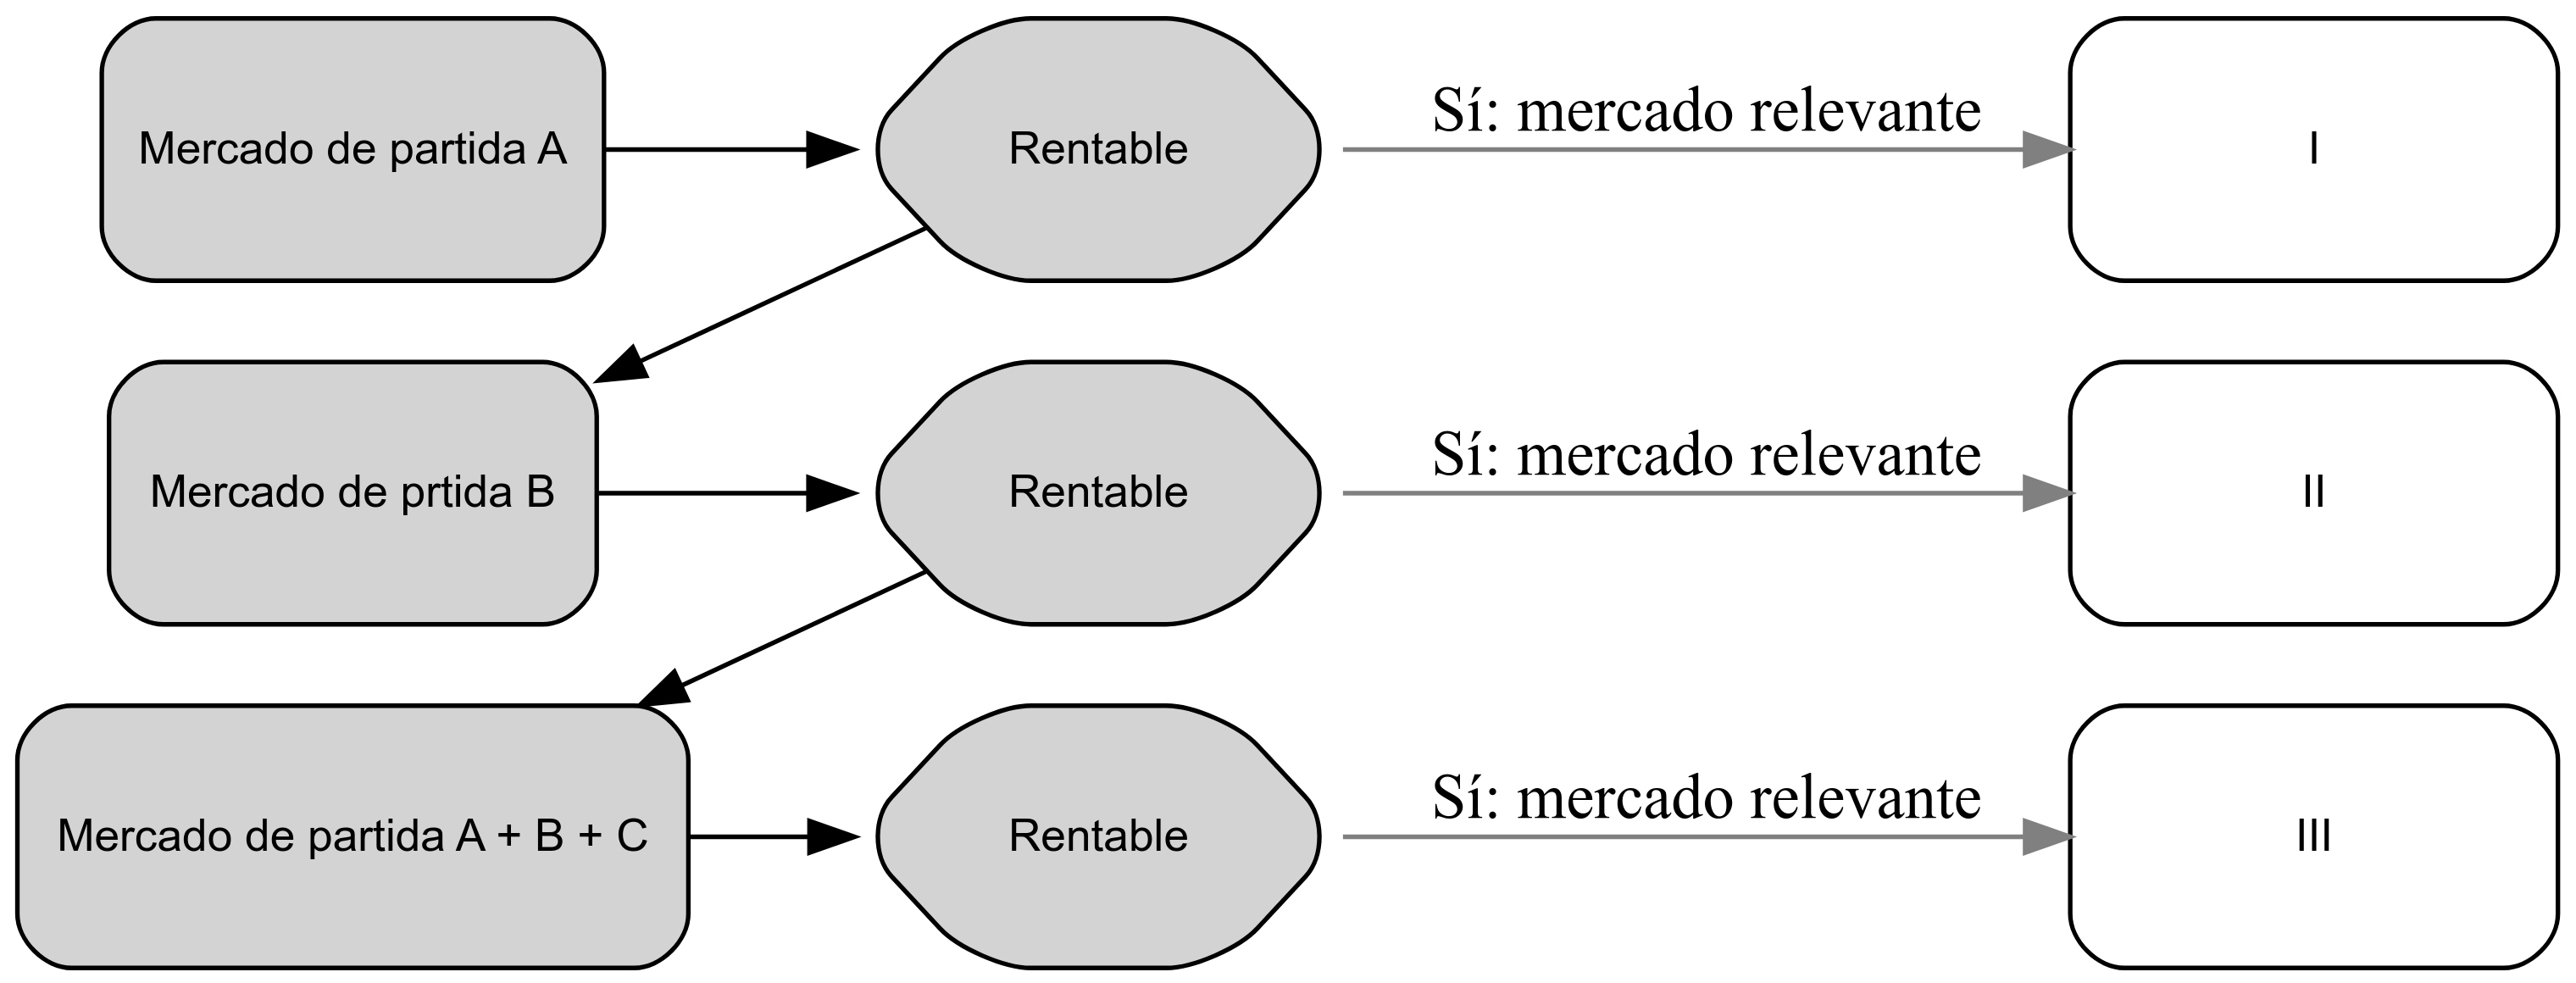
\includegraphics[width=5.5in,height=3.5in]{index_files/figure-latex/dot-figure-1.png}

}

\end{figure}

\begin{enumerate}
\def\labelenumi{\arabic{enumi}.}
\item
  ¿Puede una empresa monopólica incrementar el precio de su producto
  entre 5\% a 10\% de manera rentable?
\item
  ¿Puede una empresa monopólica que produce y vende los bienes A y B
  incrementar el precio de A y B entre 5\% y 10\% de manera rentable?
\item
  ¿Puede una empresa monopólica que produce y vende los bienes A, B y C
  incrementar el precio de A, B y C entre 5\% y 10\% de manera rentable?
\end{enumerate}

Se repite el proceso hasta conocer que ya no hay productos sustitutos.

\hypertarget{ejemplo-de-determinaciuxf3n-del-mercado-relevante-para-un-monopolista}{%
\subsubsection{Ejemplo de determinación del mercado relevante para un
monopolista}\label{ejemplo-de-determinaciuxf3n-del-mercado-relevante-para-un-monopolista}}

En este ejemplo, analizaremos la situación de una empresa monopolista,
llamada A, y evaluaremos si el mercado en el que opera es relevante.
Utilizaremos datos específicos para ilustrar el proceso.

\textbf{Datos de la empresa A}

Supongamos que la empresa A produce el bien A, con un precio inicial de
\(P_A = 10\), una cantidad producida de \(Q_A = 1000\), un costo
marginal de producción de \(CMeT_A = 5\) y una ganancia bruta de
\(B_A = 5000\).

\textbf{Incremento de precio de la empresa A}

Si la empresa A decide aumentar el precio entre un 5\% y un 10\%,
obtenemos los siguientes resultados: el precio se convierte en
\(P_A = 11\), la cantidad producida disminuye a \(Q_A = 800\), el costo
marginal de producción sigue siendo \(CMeT_A = 5\) y la ganancia bruta
se reduce a \(B_A = 4800\).

\textbf{Análisis del mercado relevante}

En este caso, al observar el efecto del incremento de precio en la
demanda de los consumidores (\(Q_A\)), podemos concluir que el mercado
no es relevante. El aumento en el precio (\(\Delta P_A\)) provoca una
sustitución de \(Q_A\) por parte de los consumidores, lo que indica que
existen otros productos que son parte del mercado relevante y son
considerados como sustitutos.

\textbf{Competidores de la empresa A}

Supongamos que la empresa A considera que sus competidores son las
empresas B y C. Sus datos son los siguientes:

\begin{itemize}
\tightlist
\item
  Empresa B: \(P_B = 13\), \(Q_B = 800\), \(CMeT_B = 4\) y
  \(B_B = 7200\).
\item
  Empresa C: \(P_C = 9\), \(Q_C = 1100\), \(CMeT_C = 4\) y
  \(B_C = 5500\).
\end{itemize}

La ganancia total en el mercado, considerando las tres empresas, es
\(B_T = 17,700\).

\textbf{Incremento de precio por parte de la empresa A}

Si el monopolista A decide aumentar el precio de su producto en un rango
del 5\% al 10\%, mientras que las otras empresas mantienen constantes
sus precios, los resultados son los siguientes:

\begin{itemize}
\tightlist
\item
  Empresa A: \(P_A = 11\), \(Q_A = 800\), \(CMeT_A = 5\) y
  \(B_A = 4800\).
\item
  Empresa B: \(P_B = 13\), \(Q_B = 900\), \(CMeT_B = 4\) y
  \(B_B = 8100\).
\item
  Empresa C: \(P_C = 9\), \(Q_C = 1200\), \(CMeT_C = 4\) y
  \(B_C = 6000\).
\end{itemize}

La ganancia total en el mercado, considerando las tres empresas, aumenta
a \(B_T = 18,900\).

\textbf{Por lo tanto:}

En este ejemplo, el monopolista A encuentra beneficioso incrementar el
precio de su producto A en un 10\%. Los consumidores sustituyen el
consumo de los otros bienes (B y C), lo que conduce a un incremento en
las ganancias totales de \$5000 a \$5400. Por lo tanto, podemos concluir
que el mercado es relevante para el producto A.

Estos ejemplos ilustran cómo se puede determinar el mercado relevante
para un monopolista, considerando los efectos de los cambios en el
precio y la demanda. Este análisis es crucial para comprender la
posición de poder de un monopolista y evaluar la competencia en el
mercado.

\begin{figure}[H]

{\centering 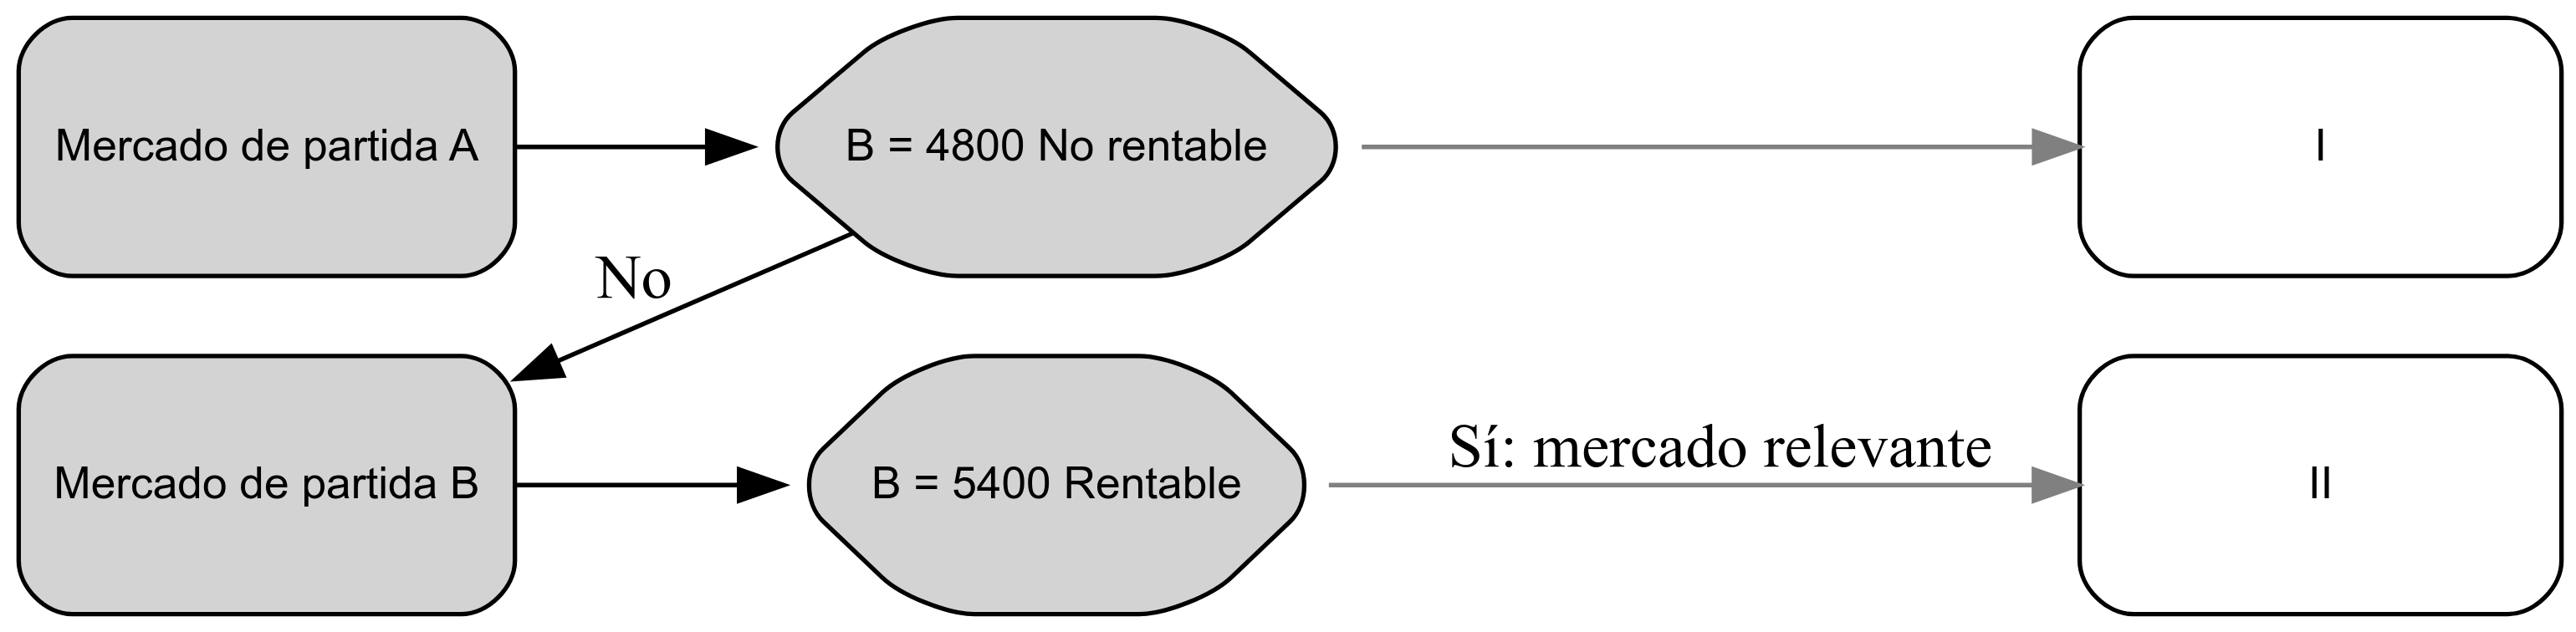
\includegraphics[width=5.5in,height=3.5in]{index_files/figure-latex/dot-figure-2.png}

}

\end{figure}

\hypertarget{elasticidad-precio-de-la-demanda-residual-de-una-empresa-con-demanda-relevante}{%
\subsection{Elasticidad Precio de la Demanda Residual de una Empresa con
Demanda
Relevante}\label{elasticidad-precio-de-la-demanda-residual-de-una-empresa-con-demanda-relevante}}

La elasticidad precio de la demanda residual es un concepto importante
en el análisis económico que permite medir la sensibilidad de la demanda
de un producto específico de una empresa ante cambios en su precio,
teniendo en cuenta los efectos de la demanda de otros productos
relacionados.

Para comprender este concepto, consideremos las siguientes ecuaciones:

La demanda total del mercado \(D_T\) se puede expresar como la demanda
del producto específico \(X_T^d\) multiplicada por el precio del
producto \(P_x\). Esta relación se muestra en la Ecuación~\ref{eq-3}:

\begin{equation}\protect\hypertarget{eq-3}{}{
D_T = X_{T}^{d} = X_{T}^{d} P_{x}
}\label{eq-3}\end{equation}

La demanda residual \(D_R\) es la demanda que queda para el producto
específico después de tener en cuenta las demandas de otros productos
relacionados. Se puede expresar como la demanda del producto residual
\(X_R^d\) multiplicada por el precio del producto \(P_x\). Esta relación
se muestra en la Ecuación~\ref{eq-4}:

\begin{equation}\protect\hypertarget{eq-4}{}{
D_R = X_R^d = X_R^d P_x
}\label{eq-4}\end{equation}

La oferta de los competidores \(S_C\) es la cantidad ofrecida por otras
empresas en el mercado, que se puede expresar como la oferta del
producto complementario \(X_C^S\) multiplicada por el precio del
producto \(P_x\). Esta relación se muestra en la Ecuación~\ref{eq-5}:

\begin{equation}\protect\hypertarget{eq-5}{}{
S_C = X_C^S = X_C^S P_x
}\label{eq-5}\end{equation}

La demanda total \(D_T\) es igual a la suma de la demanda residual
\(D_R\) y la oferta de los competidores \(S_C\). Esta relación se
muestra en la Ecuación~\ref{eq-6}:
\begin{equation}\protect\hypertarget{eq-6}{}{
D_T = D_R + S_C \equiv X_t^d = X_R^d + X_C^S \equiv X_t^d P_x = X_R^d P_x + X_C^S P_x
}\label{eq-6}\end{equation}

Donde:

\begin{itemize}
\tightlist
\item
  \(D_T\) es la demanda total del producto.
\item
  \(D_R\) es la demanda residual del producto.
\item
  \(S_C\) es la demanda de productos complementarios o sustitutos
\end{itemize}

A partir de la Ecuación~\ref{eq-6}, podemos despejar la demanda residual
\(D_R\) y obtener el siguiente:
\begin{equation}\protect\hypertarget{eq-7}{}{
X_R^d P_x = X_T^d P_x - X_C^S P_x
}\label{eq-7}\end{equation}

Aplicando la Ecuación~\ref{eq-1} a la Ecuación~\ref{eq-7}, obtenemos:

\begin{equation}\protect\hypertarget{eq-8}{}{
\frac{\partial X_R^d P_x}{\partial P_x} \frac{P_x}{X_R^d} = \frac{\partial X_T^d P_x}{\partial P_x} \frac{P_x}{X_T^d} - \frac{\partial X_C^S P_x}{\partial P_x} \frac{P_x}{X_C^S}
}\label{eq-8}\end{equation}

Multiplicando los elementos de la Ecuación~\ref{eq-8} por
\(\frac{X_T^d}{X_R^d}\) y \(\frac{X_C^S}{X_R^d}\), hacia la derecha,
obtenemos:

\begin{equation}\protect\hypertarget{eq-9}{}{
\frac{\partial X_R^d P_x}{\partial P_x} \frac{P_x}{X_R^d} = \frac{\partial X_T^d P_x}{\partial P_x} \frac{P_x}{X_T^d} \frac{X_T^d}{X_R^d} - \frac{\partial X_C^S P_x}{\partial P_x} \frac{P_x}{X_C^S} \frac{X_C^S}{X_R^d}
}\label{eq-9}\end{equation}

Dividiendo el primer elemento de la Ecuación~\ref{eq-9} tanto en el
numerador como en el denominador por \(X_T^d\), obtenemos:

\begin{equation}\protect\hypertarget{eq-10}{}{
\frac{\partial X_R^d P_x}{\partial P_x} \frac{P_x}{X_R^d} = \frac{\partial X_T^d P_x}{\partial P_x} \frac{P_x}{X_T^d} \frac{\frac{X_T^d}{X_T^d}}{\frac{X_R^d}{X_T^d}} - \frac{\partial X_C^S P_x}{\partial P_x} \frac{P_x}{X_C^S} \frac{X_C^S}{X_R^d}
}\label{eq-10}\end{equation}

Considerando que \(X_C^S = X_T^d - X_R^d\), podemos reemplazarlo en la
Ecuación~\ref{eq-10}, obteniendo :

\begin{equation}\protect\hypertarget{eq-11}{}{
\frac{\partial X_R^d P_x}{\partial P_x} \frac{P_x}{X_R^d} = \frac{\partial X_T^d P_x}{\partial P_x} \frac{P_x}{X_T^d} \frac{\frac{X_T^d}{X_T^d}}{\frac{X_R^d}{X_T^d}} - \frac{\partial X_C^S P_x}{\partial P_x} \frac{P_x}{X_C^S} \frac{X_T^d - X_R^d}{X_R^d}
}\label{eq-11}\end{equation}

En esta Ecuación~\ref{eq-11}, tienen la forma de la elasticidad precio
de la demanda, por lo que podemos reescribir la ecuación como:

\begin{equation}\protect\hypertarget{eq-12}{}{
\eta_{P_{x}X_R^d}^d = \eta_{P_{x}X_T^d}^d \frac{1}{\frac{X_R^d}{X_T^d}} - \eta_{P_{x}X_C^S}^S \frac{X_T^d - X_R^d}{X_R^d}
}\label{eq-12}\end{equation}

Ordenando y considerando que \(\frac{X_R^d}{X_T^d} = S_R\), tenemos:

\begin{equation}\protect\hypertarget{eq-13}{}{
\eta_{P_{x}X_R^d}^d = \eta_{P_{x}X_T^d}^d \frac{1}{S_R} - \eta_{P_{x}X_C^S}^S (\frac{X_T^d}{X_R^d} - 1)
}\label{eq-13}\end{equation}

Dividiendo el segundo elemento de la Ecuación~\ref{eq-13} dentro del
paréntesis tanto en el numerador como en el denominador por \(X_T^d\),
tenemos:

\begin{equation}\protect\hypertarget{eq-14}{}{
\eta_{P_{x}X_R^d}^d = \eta_{P_{x}X_T^d}^d \frac{1}{S_R} - \eta_{P_{x}X_C^S}^S (\frac{\frac{X_T^d}{X_T^d}}{\frac{X_R^d}{X_T^d}} - 1)
}\label{eq-14}\end{equation}

La Ecuación~\ref{eq-14} puede ser simplificada aún más considerando que
\(\frac{X_R^d}{X_T^d} = S_R\), obtenemos:

\begin{equation}\protect\hypertarget{eq-15}{}{
\eta_{P_{x}X_R^d}^d = \eta_{P_{x}X_T^d}^d \frac{1}{S_R} - \eta_{P_{x}X_C^S}^S (\frac{1}{S_R} - 1)
}\label{eq-15}\end{equation}

La Ecuación~\ref{eq-15} nos permite calcular la elasticidad precio de la
demanda residual de una empresa considerando las elasticidades de la
demanda del mercado y la oferta de las demás empresas. Esta medida es
importante para determinar si la elasticidad más relevante para la
empresa es la elasticidad de su demanda o la elasticidad del mercado en
general. Dependiendo de la conducta de los competidores, una u otra
elasticidad puede ser más relevante. por ejemplo:

\begin{itemize}
\tightlist
\item
  Si el precio del producto de la empresa aumenta y no es seguido por
  las otras empresas oferentes, entonces la elasticidad precio de la
  demanda de la empresa es más relevante.
\item
  Por el contrario, si el precio del producto de la empresa aumenta y es
  seguido por aumentos similares de precios por parte de los otros
  oferentes, la elasticidad más relevante para la empresa estará más
  cerca de la elasticidad precio de la demanda de mercado..
\end{itemize}

En este sentido, el análisis de la elasticidad relevante nos permite
identificar y evaluar las posibles respuestas de los competidores ante
determinadas estrategias.s.

Ordenamos la Ecuación~\ref{eq-15} obtenemos:

\begin{equation}\protect\hypertarget{eq-16}{}{
\eta_{P_{x}X_R^d}^d = \frac{\eta_{P_{x}X_T^d}^d - \eta_{P_{x}X_C^S}^{S} (1-S_R)}{S_R}
}\label{eq-16}\end{equation}

En esta Ecuación~\ref{eq-16}

\begin{itemize}
\item
  \(\eta_{P_{x}X_R^d}^d\) es la elasticidad precio de la demanda
  residual de la empresa.
\item
  \(\eta_{P_{x}X_T^d}^d\) es la elasticidad precio de la demanda del
  mercado con componente residual.
\item
  \(\eta_{P_{x}X_C^S}^S\) es la elasticidad precio de la oferta de las
  demás empresas que compiten en el mercado.
\item
  \(S_R\) es la participación de ventas de la empresa con mercado
  relevante.
\end{itemize}

\hypertarget{implicaciones-de-la-elasticidad-precio-de-la-demanda-residual}{%
\subsection{Implicaciones de la Elasticidad Precio de la Demanda
Residual}\label{implicaciones-de-la-elasticidad-precio-de-la-demanda-residual}}

\hypertarget{relaciuxf3n-entre-la-elasticidad-de-la-demanda-de-mercado-y-la-elasticidad-de-la-demanda-residual}{%
\subsubsection{1. Relación entre la Elasticidad de la Demanda de Mercado
y la Elasticidad de la Demanda
Residual}\label{relaciuxf3n-entre-la-elasticidad-de-la-demanda-de-mercado-y-la-elasticidad-de-la-demanda-residual}}

La relación entre la elasticidad precio de la demanda de mercado y la
elasticidad precio de la demanda residual puede variar. Es posible que
una demanda de mercado sea inelástica \(\eta_{P_{x}X_T^d}^d\) (baja
elasticidad precio de la demanda de mercado) pero que la demanda
residual sea elástica \(\eta_{P_{x}X_R^d}^d\) (alta elasticidad precio
de la demanda residual), siempre y cuando exista una elasticidad precio
de la oferta de las otras empresas competidoras en el mercado.

En otras palabras, incluso si la demanda de mercado en su conjunto es
relativamente insensible a los cambios de precio, la demanda específica
de la empresa puede ser más sensible. Esto se debe a que la empresa
puede enfrentar una mayor competencia por parte de otras empresas que
ofrecen productos similares, lo que aumenta la elasticidad precio de la
demanda residual de la empresa.

\hypertarget{determinaciuxf3n-de-la-elasticidad-de-la-demanda-residual-en-una-empresa-monopuxf3lica}{%
\subsubsection{2. Determinación de la Elasticidad de la Demanda Residual
en una Empresa
Monopólica}\label{determinaciuxf3n-de-la-elasticidad-de-la-demanda-residual-en-una-empresa-monopuxf3lica}}

En el caso de una empresa monopólica que opera con demanda residual, la
elasticidad de la demanda residual (\(\eta_{P_{x}X_R^d}^d\)) tiene
implicaciones importantes. Si la empresa no puede aumentar el precio de
su producto en un rango del 5\% al 10\% sin experimentar una disminución
significativa y sostenida en sus ventas, entonces se enfrenta a una
función de demanda residual elástica (alta \(\eta_{P_{x}X_R^d}^d\)).

Por otro lado, si la demanda total o de mercado es inelástica (baja
\(\eta_{P_{x}X_T^d}^d\)), esto implica que la oferta de las otras
empresas competidoras es elástica (alta \(\eta_{P_{x}X_C^S}^S\)). En
este caso, las acciones y decisiones de las otras empresas determinan el
mercado relevante en términos de oferta y competencia.

\hypertarget{ejemplo-de-un-mercado-relevante}{%
\subsection{Ejemplo de un Mercado
Relevante}\label{ejemplo-de-un-mercado-relevante}}

En este ejemplo, analizaremos un mercado relevante que involucra a tres
productos: Ron Cartavio, Pisco y Cerveza. Utilizaremos datos ficticios
para ilustrar el cálculo de los beneficios de cada producto y
examinaremos cómo se ven afectados cuando las empresas de Piscos
aumentan el precio en un 10\%.

\begin{quote}
En quechua el idioma de los incas. la palabra Pisko significa ave o
pájaro. El licor Pisco es el aguardiente obtenido por destilación de
mostos frescos de uvas pisqueras.
\end{quote}

\hypertarget{ron-cartavio}{%
\subsubsection{Ron Cartavio}\label{ron-cartavio}}

\begin{itemize}
\tightlist
\item
  Precio: \(P_r = 28\)
\item
  Cantidad: \(Q_r = 25,000\)
\item
  Costo Medio Total: \(CMeT_r = 11\)
\end{itemize}

Para calcular los beneficios (\(B_r\)) de Ron Cartavio, utilizamos la
fórmula:

\(B_r = (P_r - CMeT_r) \times Q_r\)

Sustituyendo los valores, obtenemos:

\(B_r = (28 - 11) \times 25,000\)

\(B_r = 425,000\)

Cuando las empresas de Piscos aumentan el precio en un 10\%, los nuevos
valores son:

\begin{itemize}
\tightlist
\item
  Precio: \(P_r = 31.8\)
\item
  Cantidad: \(Q_r = 21,250\)
\item
  Costo Medio Total: \(CMeT_r = 11\)
\end{itemize}

Calculando los beneficios nuevamente:

\(B_r = (31.8 - 11) \times 21,250\)

\(B_r = 420,750\)

\hypertarget{pisco}{%
\subsubsection{Pisco}\label{pisco}}

\begin{itemize}
\tightlist
\item
  Precio: \(P_{co} = 35\)
\item
  Cantidad: \(Q_{co} = 20,000\)
\item
  Costo Medio Total: \(CMeT_{co} = 15\)
\end{itemize}

Para calcular los beneficios (\(B_{co}\)) de Pisco, utilizamos la
fórmula:

\(B_{co} = (P_{co} - CMeT_{co}) \times Q_{co}\)

Sustituyendo los valores, obtenemos:

\(B_{co} = (35 - 15) \times 20,000\)

\(B_{co} = 420,000\)

Después del aumento del precio en un 10\%:

\begin{itemize}
\tightlist
\item
  Precio: \(P_{co} = 38.5\)
\item
  Cantidad: \(Q_{co} = 20,000\)
\item
  Costo Medio Total: \(CMeT_{co} = 15\)
\end{itemize}

Calculando los beneficios nuevamente:

\(B_{co} = (38.5 - 15) \times 20,000\)

\(B_{co} = 423,000\)

\hypertarget{cerveza}{%
\subsubsection{Cerveza}\label{cerveza}}

\begin{itemize}
\tightlist
\item
  Precio: \(P_c = 5\)
\item
  Cantidad: \(Q_c = 70,000\)
\item
  Costo Medio Total: \(CMeT_c = 2\)
\end{itemize}

Para calcular los beneficios (\(B_c\)) de la Cerveza, utilizamos la
fórmula:

\(B_c = (P_c - CMeT_c) \times Q_c\)

Sustituyendo los valores, obtenemos:

\(B_c = (5 - 2) \times 70,000\)

\(B_c = 210,000\)

Después del aumento del precio en un 10\%:

\begin{itemize}
\tightlist
\item
  Precio: \(P_c = 5\)
\item
  Cantidad: \(Q_c = 70,000\)
\item
  Costo Medio Total: \(CMeT_c = 2\)
\end{itemize}

Calculando los beneficios nuevamente:

\(B_c = (5 - 2) \times 70,000\)

\(B_c = 210,000\)

Por lo tanto:

\begin{itemize}
\tightlist
\item
  En el caso de Ron Cartavio, los beneficios disminuyen ligeramente
  después del aumento del precio de los Piscos.
\item
  Para Pisco, los beneficios aumentan después del aumento del precio.
\item
  En el caso de la Cerveza, los beneficios también se mantienen iguales.
\end{itemize}

\hypertarget{la-falacia-del-celofuxe1n-o-picuxf3n}{%
\subsection{La Falacia del Celofán o
Picón}\label{la-falacia-del-celofuxe1n-o-picuxf3n}}

La falacia del celofán, también conocida como falacia del picón, es un
tipo de razonamiento incorrecto que se presenta en los mercados
relevantes. Se refiere a la situación en la cual una empresa que vende
un producto con pocos sustitutos percibe erróneamente que su producto es
único en el mercado, lo que la lleva a aumentar repetidamente el precio
del producto en un 5\%, 10\% u otro porcentaje. Sin embargo, a medida
que aumenta el precio, se produce una disminución en las ventas. Esto
ocurre porque, con el aumento de los precios, otras empresas ingresan al
mercado ofreciendo bienes similares o sustitutos, lo que reduce la
demanda del producto.

\hypertarget{explicaciuxf3n-de-la-falacia-del-celofuxe1n}{%
\subsubsection{Explicación de la falacia del
celofán}\label{explicaciuxf3n-de-la-falacia-del-celofuxe1n}}

La falacia del celofán se basa en una suposición incorrecta de que un
producto no tiene sustitutos directos en el mercado. Esta suposición
lleva a la empresa a creer que puede aumentar continuamente el precio
sin perder clientes. Sin embargo, a medida que el precio se eleva, los
consumidores comienzan a buscar alternativas similares y sustitutas, lo
que reduce la demanda del producto original.

Además, la elasticidad cruzada de la demanda de los bienes sustitutos
juega un papel importante en esta falacia. Si la elasticidad cruzada de
la demanda es baja, significa que los consumidores tienen dificultades
para encontrar y adoptar sustitutos cuando el precio de un producto
aumenta. Esto permite que la empresa incremente los precios sin
enfrentar una disminución significativa en la demanda. Sin embargo, en
algún punto, cuando los precios alcanzan un nivel crítico, los
consumidores comienzan a buscar alternativas y la demanda del producto
original se reduce.

\hypertarget{consideraciones-para-los-monopolistas}{%
\subsubsection{Consideraciones para los
monopolistas}\label{consideraciones-para-los-monopolistas}}

Para los monopolistas, una de las preocupaciones principales es evitar
que sus productos sean sustituidos por otros similares en el mercado.
Por lo tanto, la sustituibilidad de sus productos debe ser
cuidadosamente evaluada, asumiendo un precio competitivo para el bien
analizado. Es fundamental conocer y analizar detalladamente la curva de
demanda, especialmente a través de las elasticidades.

Por ejemplo, si se opera en la parte elástica de una curva de demanda
inicialmente inelástica, a medida que se incrementa el precio del
producto, la demanda se vuelve más elástica y, en consecuencia, la
cantidad demandada disminuye. En este sentido, la estrategia de aumentar
los precios para ampliar la demanda, siguiendo la estrategia de un
monopolista, no es una política efectiva para lograr dicho objetivo.

\hypertarget{otras-formas-de-competir-y-permanecer-en-el-mercado-relevante}{%
\subsection{Otras Formas de Competir y Permanecer en el Mercado
Relevante}\label{otras-formas-de-competir-y-permanecer-en-el-mercado-relevante}}

Existe diversas estrategias que las empresas pueden emplear para
competir y mantenerse en el mercado relevante. Estas estrategias van más
allá de la simple fijación de precios y se centran en aspectos clave
como el diseño de productos, la comprensión de las preferencias de los
consumidores, el análisis de productos sustitutos y la optimización de
costos, tecnología, inversión e investigación.

\hypertarget{diseuxf1o-y-comparaciuxf3n-de-productos}{%
\subsubsection{Diseño y Comparación de
Productos}\label{diseuxf1o-y-comparaciuxf3n-de-productos}}

Una forma efectiva de competir en el mercado relevante es a través del
diseño y la comparación de productos. Esto implica desarrollar productos
con características únicas y atractivas que los diferencien de los
competidores. Además, es importante realizar un análisis comparativo con
los productos existentes en el mercado para identificar fortalezas y
debilidades y destacar las ventajas competitivas.

El diseño de productos innovadores y la capacidad de comunicar
claramente sus beneficios pueden generar una demanda adicional y atraer
a los consumidores que valoran las características distintivas. Es
fundamental entender las necesidades y deseos de los clientes para
adaptar el diseño y ofrecer un producto que satisfaga sus expectativas.

\hypertarget{identificaciuxf3n-de-gustos-preferencias-y-patrones-de-consumo}{%
\subsubsection{Identificación de Gustos, Preferencias y Patrones de
Consumo}\label{identificaciuxf3n-de-gustos-preferencias-y-patrones-de-consumo}}

Otra estrategia es la identificación de los gustos, preferencias y
patrones de consumo de los consumidores. Esto se logra a través de
investigaciones de mercado, análisis de datos y seguimiento de
tendencias. Al comprender a fondo a los clientes, las empresas pueden
ajustar sus estrategias de marketing y adaptar sus productos para
satisfacer sus necesidades específicas.

La recopilación de información demográfica, comportamiento de compra,
preferencias de marca y opiniones del consumidor permite segmentar el
mercado y personalizar las ofertas. Esto facilita la creación de
campañas publicitarias más efectivas, la mejora de la experiencia del
cliente y la construcción de relaciones duraderas con los consumidores.

\hypertarget{pruxe1cticas-de-regresiuxf3n-y-correlaciuxf3n-entre-productos-sustitutos}{%
\subsubsection{Prácticas de Regresión y Correlación entre Productos
Sustitutos}\label{pruxe1cticas-de-regresiuxf3n-y-correlaciuxf3n-entre-productos-sustitutos}}

La aplicación de técnicas estadísticas como la regresión y la
correlación puede proporcionar información valiosa sobre los productos
sustitutos en el mercado. Estas prácticas permiten identificar la
relación entre variables y determinar qué factores pueden influir en la
demanda de un producto en particular.

Al analizar las interacciones entre productos sustitutos, las empresas
pueden comprender mejor cómo los cambios en el precio, la calidad o las
promociones de un producto afectan la demanda de otros productos
similares. Esto proporciona información estratégica para ajustar la
oferta, establecer precios competitivos y anticipar las respuestas de
los consumidores ante cambios en el mercado.

\hypertarget{competencia-minimizando-costos-tecnologuxeda-inversiuxf3n-e-investigaciuxf3n}{%
\subsubsection{Competencia Minimizando Costos, Tecnología, Inversión e
Investigación}\label{competencia-minimizando-costos-tecnologuxeda-inversiuxf3n-e-investigaciuxf3n}}

Para mantenerse en el mercado relevante, las empresas también deben
competir eficientemente minimizando costos, aprovechando la tecnología,
realizando inversiones inteligentes e impulsando la investigación y el
desarrollo. Estas prácticas permiten mejorar la productividad, la
calidad y la innovación, lo que puede brindar una ventaja competitiva
sostenible.

La optimización de los costos operativos, la implementación de
tecnologías avanzadas, las inversiones estratégicas en recursos clave y
el fomento de la investigación y el desarrollo son fundamentales para
garantizar la eficiencia y la adaptabilidad en un entorno empresarial
dinámico. Estas prácticas pueden ayudar a las empresas a ofrecer
productos de alta calidad a precios competitivos, mejorar la
satisfacción del cliente y mantener una posición sólida en el mercado
relevante.

\begin{quote}
Hay competencia en muchos otros productos
\end{quote}

\hypertarget{mercado-del-producto-relevante-por-el-lado-de-la-oferta}{%
\section{Mercado del Producto Relevante por el Lado de la
Oferta}\label{mercado-del-producto-relevante-por-el-lado-de-la-oferta}}

\hypertarget{elasticidad-precio-de-la-oferta}{%
\subsection{Elasticidad Precio de la
Oferta}\label{elasticidad-precio-de-la-oferta}}

Un mercado de producto es considerado relevante por el lado de la oferta
si la elasticidad precio de la oferta es alta, lo que implica que la
oferta es elástica. La elasticidad precio de la oferta se define como la
medida de la sensibilidad de la cantidad ofrecida de un bien ante
cambios en su precio. Si la elasticidad precio de la oferta es alta,
significa que la cantidad ofrecida cambia significativamente en
respuesta a cambios en el precio.

\begin{equation}\protect\hypertarget{eq-17}{}{
\eta_{XP_{y}} = \frac{\partial X^s}{\partial P_{x}} \frac{P_{x}}{X}
}\label{eq-17}\end{equation}

\begin{equation}\protect\hypertarget{eq-18}{}{
\eta_{XP_{y}} = \frac{\frac{\Delta X^s}{X}}{\frac{\Delta P_{x}}{P_{x}}}
}\label{eq-18}\end{equation}

Las ecuaciones presentadas nos permiten calcular la elasticidad precio
de la oferta. La Ecuación~\ref{eq-17} muestra la fórmula general, donde
\(X^s\) representa la cantidad ofrecida del bien, \(P_x\) es el precio
del bien y \(X\) es la cantidad total del bien. La Ecuación~\ref{eq-18}
muestra una forma simplificada de calcular la elasticidad precio de la
oferta utilizando cambios porcentuales.

\hypertarget{ampliaciuxf3n-del-mercado-relevante}{%
\subsection{Ampliación del Mercado
Relevante}\label{ampliaciuxf3n-del-mercado-relevante}}

En el largo plazo, es posible que se permita la entrada de nuevas
empresas que producen bienes sustitutos a bajos costos. Esto implica la
ampliación del mercado relevante, ya que se incluiría a este nuevo grupo
de empresas en el mercado futuro. La entrada de nuevas empresas con
bienes sustitutos puede tener un impacto significativo en la competencia
y en la dinámica del mercado, ya que proporciona a los consumidores más
opciones y puede influir en los precios y la calidad de los productos.

\hypertarget{factores-que-limitan-el-mercado-geogruxe1fico-relevante}{%
\subsection{Factores que Limitan el Mercado Geográfico
Relevante}\label{factores-que-limitan-el-mercado-geogruxe1fico-relevante}}

Existen varios factores que limitan el alcance geográfico del mercado
relevante y que deben tenerse en cuenta al evaluar las posibilidades de
aprovisionamiento de bienes sustitutos. Algunos de estos factores son:

\begin{enumerate}
\def\labelenumi{\arabic{enumi}.}
\item
  Disponibilidad de Proveedores Alternativos: Es importante evaluar si
  existen proveedores alternativos que puedan atender a los clientes en
  el mercado relevante. Esto implica analizar la capacidad y disposición
  de estos proveedores para satisfacer la demanda.
\item
  Capacidad de Abastecimiento del Cliente: El cliente debe tener la
  capacidad de abastecerse de distintos proveedores en caso de
  necesidad. Esto puede incluir consideraciones logísticas, como la
  disponibilidad de transporte y la distancia geográfica entre el
  cliente y los proveedores alternativos.
\item
  Seguridad y Confianza: El cliente también puede tener inquietudes
  relacionadas con la seguridad y la confianza al acudir a un mercado
  geográficamente relevante. Debe evaluarse la garantía de encontrar el
  producto deseado, así como el costo y el tiempo de demora asociados
  con el acceso a ese mercado.
\end{enumerate}

Es fundamental considerar estos factores al determinar el mercado
geográfico relevante y evaluar las opciones disponibles para los
consumidores en términos de precios, calidad y disponibilidad de
productos sustitutos.

\hypertarget{definiciuxf3n-de-mercado-geogruxe1fico-relevante-en-el-peruxfa}{%
\section{Definición de Mercado Geográfico Relevante en el
Perú}\label{definiciuxf3n-de-mercado-geogruxe1fico-relevante-en-el-peruxfa}}

\hypertarget{definiciuxf3n-seguxfan-la-resoluciuxf3n-n-0078-1999dtc-indecopi}{%
\subsection{Definición según la Resolución N 0078-1999/DTC --
INDECOPI}\label{definiciuxf3n-seguxfan-la-resoluciuxf3n-n-0078-1999dtc-indecopi}}

La Resolución N 0078-1999/DTC -- INDECOPI, emitida el 5 de marzo de
1999, establece que el mercado geográfico relevante se refiere a las
fuentes alternativas de aprovisionamiento a las que puede acudir el
consumidor o usuario en el corto plazo si el precio del producto o
servicio se incrementa de manera significativa. Esta definición enfatiza
la importancia de identificar las opciones disponibles para los
consumidores en caso de un aumento de precio considerable.

\hypertarget{definiciuxf3n-seguxfan-la-resoluciuxf3n-n-117-97-tdc}{%
\subsection{Definición según la Resolución N
117-97-TDC}\label{definiciuxf3n-seguxfan-la-resoluciuxf3n-n-117-97-tdc}}

La Resolución N 117-97-TDC, emitida el 5 de mayo de 1997, proporciona
una perspectiva adicional sobre la determinación del mercado relevante.
Según esta resolución, para determinar el mercado relevante se deben
examinar las fuentes de aprovisionamiento a las que un comprador puede
acudir. Es importante considerar las alternativas reales disponibles en
función del nivel de sustitución entre productos, así como los costos
asociados con esas alternativas para el proveedor.

\hypertarget{explicaciuxf3n-de-los-conceptos}{%
\subsection{Explicación de los
Conceptos}\label{explicaciuxf3n-de-los-conceptos}}

La definición de mercado geográfico relevante se centra en identificar
las fuentes alternativas de aprovisionamiento a las que pueden recurrir
los consumidores en caso de un aumento significativo en el precio de un
producto o servicio. Es decir, se busca determinar qué otras opciones
tienen los consumidores en el corto plazo si el precio de un producto o
servicio se vuelve menos atractivo.

La noción de sustitución entre productos es crucial para comprender el
mercado relevante. Se refiere a la capacidad de los consumidores para
satisfacer una misma necesidad o deseo utilizando diferentes productos o
servicios. Cuanto mayor sea el nivel de sustitución entre productos, es
decir, cuanto más similares y competitivos sean los productos entre sí,
mayor será el alcance del mercado relevante.

Además, al determinar el mercado relevante, es fundamental considerar
los costos asociados con las alternativas disponibles para los
proveedores. Esto implica evaluar los costos de producción, distribución
y otros factores que puedan influir en la viabilidad de las fuentes
alternativas de aprovisionamiento.


\printbibliography


\end{document}
